\documentclass[11pt,a4paper]{amsart}
\usepackage[utf8]{inputenc}
\usepackage[T1]{fontenc}
\usepackage{amsmath,amssymb,amsthm}
\usepackage{graphicx}
\usepackage{booktabs}
\usepackage{longtable}
\usepackage[margin=2.6cm]{geometry}
\usepackage[colorlinks=true,linkcolor=blue,citecolor=blue,urlcolor=blue]{hyperref}

\newtheorem{theorem}{Theorem}
\newtheorem{lemma}[theorem]{Lemma}
\newtheorem{proposition}[theorem]{Proposition}
\newtheorem{corollary}[theorem]{Corollary}
\theoremstyle{remark}
\newtheorem{remark}[theorem]{Remark}

\newcommand{\Q}{\mathbb{Q}}
\newcommand{\R}{\mathbb{R}}
\newcommand{\F}{\mathbb{F}}
\newcommand{\Euc}{\mathrm{E}(2)}

\title[Two forbidden distances $1$ and $(\sqrt2+\sqrt6)/2$]{The plane with forbidden distances $1$ and $(\sqrt2+\sqrt6)/2$\\ needs at least seven colours}
\author{Chrysovalantis Tsirindanis}
\address{School of Electrical and Computer Engineering, National Technical University of Athens, Greece}
\date{\today}

\begin{document}

\begin{abstract}
Let $d=(\sqrt2+\sqrt6)/2$. We prove that every colouring of the plane in which no two points at distance $1$ or $d$ share a colour uses at least $7$ colours. The bound $\chi\ge7$ was obtained in outline in the Polymath16 discussion in 2019, from an $8$-point gadget of Parts and an observation of de Grey, but no complete proof or explicit certificate was ever written down. Our proof follows that outline and combines the averaging (invariant mean) method of P\'alv\"olgyi and \'Agoston with a finite certificate: a configuration of $262$ points in $\Q(i,\sqrt3,\sqrt7)$ with $248$ isosceles triangles for which a constraint system is unsatisfiable. The certificate is checked by exact arithmetic and by a machine-verified resolution proof of $602{,}287$ steps. Together with the standard upper bound, $7\le\chi(\{1,d\})\le12$. The proof does not use the strict inequality $p_\delta<\tfrac12$ for six colours, for which only a sketch is available. We also give a vertex-critical $6$-chromatic $\{1,d\}$-graph with $30$ vertices (the previous smallest known has $117$) and show that every finite $\{1,d\}$-graph in $\Q(i,\sqrt3)$ is $4$-colourable.
\end{abstract}

\maketitle

\section{Introduction}

For $d>1$ let $\chi(\{1,d\})$ be the least number of colours for the Euclidean plane such that no two points at distance $1$ or $d$ share a colour. A finite point set, joined when the distance is $1$ or $d$, is a \emph{$\{1,d\}$-graph}.

The bound $\chi(\{1,d\})\ge6$ is known for $d=2$ (Exoo--Ismailescu~\cite{EI19}), $d=(1+\sqrt5)/2$ (Huddleston; a $16$-vertex proof is due to Parts~\cite{Pa20}), and $d=\sqrt3$ and $d=(\sqrt3+1)/\sqrt2=(\sqrt2+\sqrt6)/2$. For the last two values P\'alv\"olgyi and \'Agoston first proved it by a probabilistic argument~\cite{Pa20}, and De Neve, Vanden Kerchove, Colle, Tavernier and Pickavet gave explicit graphs with $33$ and $117$ vertices~\cite{DN25}. For $d=(\sqrt2+\sqrt6)/2$, $\chi\ge7$ was argued in outline in the fifteenth Polymath16 thread~\cite{PM15}: Parts proposed the $8$-point gadget of Lemma~\ref{lem:gadget} (24 December 2019), and de Grey observed that if some $p_\delta=\tfrac12$ then every isosceles triangle with legs $\delta$ and base $1$ has a monochromatic leg (28 December 2019). The gadget appears there only as an image, the argument only in words, and according to~\cite{DN25} many details are missing.

Throughout, $d=(\sqrt2+\sqrt6)/2$, so $d^2=2+\sqrt3$.

\begin{theorem}\label{thm:seven}
$\chi(\{1,(\sqrt2+\sqrt6)/2\})\ge7$.
\end{theorem}

The shortest route to Theorem~\ref{thm:seven} combines the gadget with the strict inequality $p_\delta<\tfrac12$ for the probability $p_\delta$ that two random points at distance $\delta>\tfrac12$ share a colour. That inequality was sketched for any number of colours by P\'alv\"olgyi in the twelfth Polymath16 thread~\cite{PM12}; \'Agoston proved it for $4$ colours and remarked that a chain of isosceles triangles extends it to any number~\cite[Prop.~4.2.6, Rem.~4.2.7]{Ag21}. No written proof for six colours is available, and we do not use it. Instead we make de Grey's observation effective. If $\chi\le6$, the gadget forces $p_{\sqrt2}=p_{1+\sqrt3}=\tfrac12$ exactly, this equality imposes a rigid rule on every isosceles triangle of the relevant shapes, and a finite configuration on which the rule cannot be satisfied (Proposition~\ref{prop:cert}) gives the contradiction. Our contribution to Theorem~\ref{thm:seven} is thus a complete, checkable proof of an argument outlined in Polymath16.

\begin{theorem}\label{thm:g30}
There is a vertex-critical $6$-chromatic $\{1,d\}$-graph $G_{30}$ with $30$ vertices and $103$ edges, all of whose vertices lie in $\Q(i,\sqrt3,\sqrt7)$.
\end{theorem}

The previously smallest known $6$-chromatic $\{1,d\}$-graph has $117$ vertices~\cite{DN25}. Finally, Proposition~\ref{prop:zeta12} shows that every finite $\{1,d\}$-graph with vertices in $\Q(i,\sqrt3)$ is $4$-colourable. This explains why the rotation $\omega=(3+i\sqrt7)/4$ appears in all three constructions.

\section{The averaging framework}\label{sec:avg}

Let $c\colon\R^2\to\{1,\dots,k\}$ be a colouring with no monochromatic pair at distance $1$ or $d$. Let $\Euc$ be the group of isometries of the plane, viewed as a discrete group. It is solvable ($\R^2\rtimes O(2)$ with $O(2)=SO(2)\rtimes C_2$), hence amenable as a discrete group~\cite{Ru02}. So there is a left-invariant mean on $\ell^\infty(\Euc)$; composing it with the inversion $g\mapsto g^{-1}$ gives a mean $\mu$ (a positive linear functional with $\mu(1)=1$) that is invariant under right translation, $\mu(f(\cdot\,h))=\mu(f)$. Equivalently, $\mu$ is a finitely additive probability measure defined on all subsets of $\Euc$; this is the setting of \'Agoston~\cite[\S4.1]{Ag21}, who uses a left-invariant measure on $S_k\times\Euc$ and the random colouring $c\circ T^{-1}$. No measurability of $c$ is assumed. For points $A,B$ put
\[
f_{A,B}(g)=\mathbf 1\bigl[c(gA)=c(gB)\bigr],\qquad g\in\Euc .
\]
Then $f_{hA,hB}(g)=f_{A,B}(gh)$, so $\mu(f_{A,B})$ depends only on $|AB|$; write $p_{|AB|}$. We use only three properties of $\mu$: linearity, positivity, and $\mu(1)=1$. In particular, if $\sum_j f_j\ge m$ pointwise then $\sum_j\mu(f_j)\ge m$.

\begin{lemma}[{\cite[Prop.~4.2.1]{Ag21}}]\label{lem:half}
For every $k$ and every $\delta\ge\tfrac12$, $p_\delta\le\tfrac12$.
\end{lemma}

\begin{proof}
Take $P,Q,R$ with $|PQ|=|PR|=\delta$ and $|QR|=1$. Since $c(gQ)\ne c(gR)$ for every $g$, $f_{P,Q}+f_{P,R}\le1$, so $2p_\delta\le1$.
\end{proof}

\begin{lemma}[gadget]\label{lem:gadget}
Let $\zeta=e^{i\pi/6}$ and $X=\{0,\,1,\,i,\,1+\zeta,\,1+i,\,\zeta^5,\,\zeta^{10},\,\zeta^2+i\}\subset\mathbb C$. All $28$ pairs of $X$ except the four pairs
\[
(1,i),\quad(1+i,0),\quad(1+\zeta,\zeta^5),\quad(\zeta^{10},\zeta^2+i)
\]
are at distance $1$ or $d$. The first two of these pairs are at distance $\sqrt2$ and the last two at distance $1+\sqrt3$. Consequently, if $k=6$ then $2p_{\sqrt2}+2p_{1+\sqrt3}\ge2$.
\end{lemma}

\begin{proof}
The distances are checked by direct computation (we verified them in exact arithmetic). For each $g$, the map $x\mapsto c(gx)$ properly colours the graph on $X$ whose edges are the $24$ forbidden pairs. Its complement is a perfect matching, so each colour class has at most two points, and a class with two points is one of the four matched pairs. Eight points in at most six classes give at least two such classes. Hence the four indicators sum to at least $2$ pointwise, and we apply $\mu$.
\end{proof}

\begin{corollary}\label{cor:equal}
If $k=6$, then $p_{\sqrt2}=p_{1+\sqrt3}=\tfrac12$.
\end{corollary}

\begin{proof}
Combine Lemmas~\ref{lem:half} and~\ref{lem:gadget}.
\end{proof}

\section{Proof of Theorem~\ref{thm:seven}}

Call a triple $(P;Q,R)$ of points a \emph{rigid triangle} if $|PQ|=|PR|\in\{\sqrt2,\,1+\sqrt3\}$ and $|QR|\in\{1,d\}$.

\begin{lemma}\label{lem:finite}
Suppose $k=6$. Let $F$ be a finite point set and $\mathcal T$ a finite set of rigid triangles with vertices in $F$. Then there is a colouring $\phi\colon F\to\{1,\dots,6\}$ such that
\begin{enumerate}
\item $\phi(x)\ne\phi(y)$ whenever $|xy|\in\{1,d\}$, and
\item $\phi(P)=\phi(Q)$ or $\phi(P)=\phi(R)$ for every $(P;Q,R)\in\mathcal T$.
\end{enumerate}
\end{lemma}

\begin{proof}
Fix $t=(P;Q,R)\in\mathcal T$ and let $\delta=|PQ|$. Because $|QR|\in\{1,d\}$, $f_{P,Q}f_{P,R}=0$, so $N_t:=1-f_{P,Q}-f_{P,R}$ takes values in $\{0,1\}$. By Corollary~\ref{cor:equal}, $\mu(N_t)=1-2p_\delta=0$. If every $g$ had $N_t(g)=1$ for some $t$, then $\sum_t N_t\ge1$ pointwise and $0=\sum_t\mu(N_t)\ge1$, which is absurd. Pick $g$ with $N_t(g)=0$ for all $t$ and set $\phi(x)=c(gx)$.
\end{proof}

\begin{proposition}\label{prop:cert}
There is a set $F$ of $262$ points in $\Q(i,\sqrt3,\sqrt7)$ and a set $\mathcal T$ of $248$ rigid triangles with vertices in $F$ for which no colouring $\phi$ as in Lemma~\ref{lem:finite} exists.
\end{proposition}

The configuration and its verification are described in Section~\ref{sec:cert}.

\begin{proof}[Proof of Theorem~\ref{thm:seven}]
A proper $6$-colouring of the plane would, by Lemma~\ref{lem:finite}, give a colouring $\phi$ of the set $F$ of Proposition~\ref{prop:cert}, which does not exist. A colouring with fewer than $6$ colours is in particular a $6$-colouring.
\end{proof}

\begin{remark}
The $\{1,d\}$-graph on $F$ alone is $6$-colourable (an explicit colouring was found and checked). Thus neither ingredient suffices by itself: the averaging argument supplies the triangle constraints, and the finite set makes them contradictory.
\end{remark}

\section{The certificate}\label{sec:cert}

Let $\omega=(3+i\sqrt7)/4$, a unit complex number of argument $\arccos(3/4)$. For a rigid triangle with legs $\sqrt2$ and base $1$ the apex angle is exactly $\arg\omega$, so such triangles need $\sqrt7$. In fact the field $\Q(\zeta)=\Q(i,\sqrt3)$ contains no rigid triangle: the apex angle $\theta$ of a rigid triangle has $\cos\theta\in\{\tfrac34,\tfrac{2+\sqrt3}4,\tfrac{2-\sqrt3}4\}$, and $e^{i\theta}=(R-P)/(Q-P)$ would lie in $\Q(\zeta)$, forcing $\sin\theta\in\Q(\sqrt3)$; but $16\sin^2\theta\in\{7,\,9-4\sqrt3,\,9+4\sqrt3\}$, none of which is a square in $\Q(\sqrt3)$.

\medskip\noindent\textbf{Construction.} Let $U=\{\zeta^k\omega^a:0\le k<12,\ a\in\{-1,0,1\}\}$ ($36$ unit vectors) and $U_d=(1+\zeta)U$ ($36$ vectors of length $d$, since $|1+\zeta|^2=2+\sqrt3$). The set $B$ of sums of at most two elements of $U\cup U_d$ has $2{,}233$ points, $21{,}936$ pairs at distance $1$ or $d$, and $2{,}064$ rigid triangles. The constraint system of Lemma~\ref{lem:finite} on $B$ is unsatisfiable. Iterated unsatisfiable-core extraction, first over triangles and then over points, reduces it to $|F|=262$ points with all $1{,}734$ pairs at distance $1$ or $d$ and $|\mathcal T|=248$ rigid triangles. The points, edges and triangles are listed in the accompanying file \texttt{cert7.json}; each point is given as a sum of at most two generators.

\medskip\noindent\textbf{Encoding.} Variables $x_{v,j}$ ($v\in F$, $1\le j\le6$) with exactly-one constraints per point; $\neg x_{u,j}\vee\neg x_{v,j}$ for every edge $uv$ and colour $j$; auxiliary variables $y_{uv,j}\Rightarrow x_{u,j}\wedge x_{v,j}$; and for every $(P;Q,R)\in\mathcal T$ the clause $\bigvee_j y_{PQ,j}\vee\bigvee_j y_{PR,j}$. The colours of one edge are fixed, which is harmless since all constraints are invariant under permuting colours. This gives $4{,}440$ variables and $20{,}582$ clauses.

\medskip\noindent\textbf{Verification.}

\begin{center}
\small
\begin{tabular}{p{3.4cm}p{8.3cm}l}
\toprule
Claim & Method & Result\\
\midrule
Edges & Exact arithmetic in PARI/GP over $\Q(\sqrt3,\sqrt7)=\Q(t)$, $t^4-20t^2+16=0$, on real and imaginary parts & $1734/1734$\\
Triangles & Same: legs equal and in $\{2,\,4+2\sqrt3\}$ (squared), base in $\{1,\,2+\sqrt3\}$ & $248/248$\\
Gadget (Lemma~\ref{lem:gadget}) & Same, all $28$ pairs & correct\\
Unsatisfiability & CNF rebuilt from \texttt{cert7.json} alone; CaDiCaL~1.9.5 refutes it in $44$\,s and emits a DRUP proof & UNSAT\\
Proof check & Independent forward RUP checker in C (\texttt{rup\_checker.c}); every one of the $602{,}287$ lemmas is RUP and the empty clause is derived & verified\\
\bottomrule
\end{tabular}
\end{center}

\noindent The checker was validated on a correct proof (accepted) and on a truncated proof (rejected). Honouring deletions only weakens the clause database, so it is sound for refutations.

\section{A $30$-vertex $6$-chromatic graph}

Starting from the $2{,}233$-point set $B$ and the plain $5$-colouring CNF (no triangles), unsatisfiable-core extraction followed by vertex deletion gives the graph $G_{30}$ of Theorem~\ref{thm:g30} (Figure~\ref{fig:g30}, Appendix~\ref{app:g30}). Every vertex has the form $(a_0+a_1\sqrt3+a_2\sqrt7+a_3\sqrt{21})/8+i(b_0+b_1\sqrt3+b_2\sqrt7+b_3\sqrt{21})/8$ with $a_j,b_j\in\mathbb Z$. It has $49$ edges of length $1$ and $54$ of length $d$, minimum degree $5$, and is the full distance graph of its vertices. The edge lengths were checked twice in exact arithmetic (SymPy and PARI/GP); non-$5$-colourability by a DRUP proof of $15{,}574$ lemmas checked by two independent RUP checkers; $6$-colourability and vertex-criticality by explicit colourings checked edge by edge.

\begin{figure}[ht]
\centering
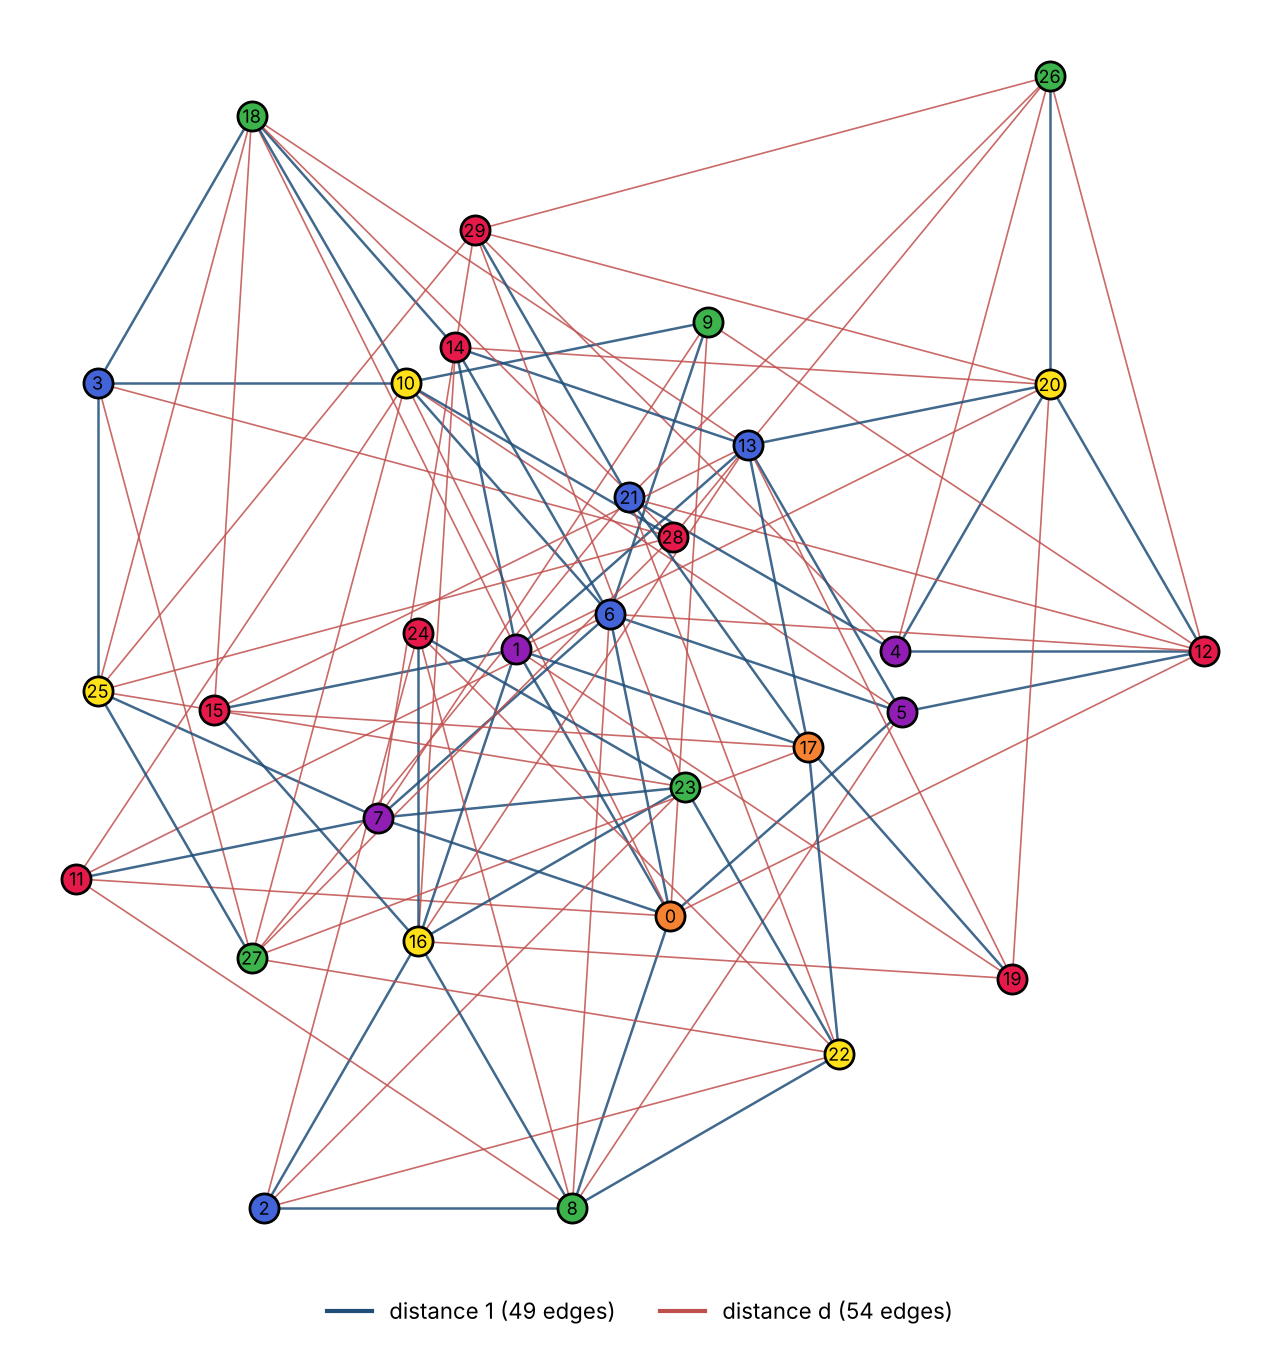
\includegraphics[width=0.66\textwidth]{g30.png}
\caption{$G_{30}$ at its true coordinates. Blue: distance $1$ ($49$ edges); red: distance $d$ ($54$ edges). Vertex colours: the $6$-colouring of Appendix~\ref{app:g30}.}
\label{fig:g30}
\end{figure}

\section{Why $\Q(i,\sqrt3)$ is not enough}

\begin{lemma}\label{lem:reduction}
Let $K$ be a CM field with maximal real subfield $K^+$, and $\delta>0$ with $\delta^2\in K^+$. Let $\mathfrak P$ be a prime of $K^+$ inert in $K/K^+$ with residue field $\F_q$, such that $\delta^2$ is a $\mathfrak P$-unit. Then every finite $\{1,\delta\}$-graph with vertices in $K$ maps homomorphically to
\[
H(q,c)=\operatorname{Cay}\bigl(\F_{q^2},\{x:x^{q+1}=1\}\cup\{x:x^{q+1}=c\}\bigr),\qquad c=\delta^2\bmod\mathfrak P.
\]
\end{lemma}

\begin{proof}
Let $\mathfrak p$ be the unique prime of $K$ over $\mathfrak P$; complex conjugation fixes it. An edge vector $v$ has $v\bar v\in\{1,\delta^2\}$, a $\mathfrak P$-unit, and $v,\bar v$ have equal $\mathfrak p$-valuation, so $v$ is a $\mathfrak p$-unit and reduces to a nonzero $x\in\F_{q^2}$. Conjugation induces Frobenius, so $x^{q+1}\in\{1,c\}$. Translating a vertex of each component to $0$ makes all vertices $\mathfrak p$-integral, and reduction is the homomorphism.
\end{proof}

\begin{proposition}\label{prop:zeta12}
Every finite $\{1,d\}$-graph with vertices in $\Q(i,\sqrt3)$ is $4$-colourable; the same holds for $\{1,\sqrt3\}$-graphs.
\end{proposition}

\begin{proof}
The prime $(1+\sqrt3)$ of $\Q(\sqrt3)$ has residue field $\F_2$ and is inert in $\Q(i,\sqrt3)$, and $2+\sqrt3$ and $3$ are units there. In $\F_4$ every nonzero element has norm $1$, so $H(2,c)=K_4$.
\end{proof}

In particular the gadget of Lemma~\ref{lem:gadget}, which lies in $\Q(\zeta)$, is $4$-colourable as a graph ($K_8$ minus a perfect matching), and no finite-graph proof of $\chi(\{1,d\})\ge5$ can live in $\Q(\zeta)$.

\begin{proposition}\label{prop:mod8}
Let $m\ge1$ be squarefree with $3\nmid m$, $K^+=\Q(\sqrt3,\sqrt m)$ and $K=K^+(i)$. The primes of $K^+$ above $2$ have residue field $\F_2$ and are inert in $K/K^+$ if and only if $m\equiv1,2,3,6\pmod 8$. In that case every finite $\{1,d\}$-graph and every finite $\{1,\sqrt3\}$-graph with vertices in $K$ is $4$-colourable.
\end{proposition}

\begin{proof}
All primes above $2$ are conjugate, so it suffices to look at one completion. The square classes of $\Q_2^\times$ are represented by $\pm1,\pm2,\pm5,\pm10$, and $\Q_2(\sqrt a)$ ($a\not\sim1$) is unramified exactly when $a\sim5$. Since $-15\equiv1\pmod8$ is a square in $\Q_2$, $3\sim-5$. Let $V\subset\Q_2^\times/\Q_2^{\times2}$ be generated by $-5$ and $m$; the completion of $K^+$ is $L=\Q_2(\sqrt V)$, and that of $K$ is $L(\sqrt{-1})$. A multiquadratic extension $\Q_2(\sqrt W)$ has residue degree $2$ if $5\in W$ and $1$ otherwise. So the residue field of $L$ is $\F_2$ iff $5\notin V$, and $L(\sqrt{-1})/L$ is inert iff moreover $-1\notin V$ and $5\in\langle V,-1\rangle$. The last condition always holds, since $-5\in V$. Now $V=\{1,-5,m,-5m\}$, and $5\notin V$, $-1\notin V$ together say $m\not\sim5$ and $m\not\sim-1$. For odd $m$ the class of $m$ is that of $m\bmod 8\in\{1,3,5,7\}$, with $3\sim-5$ and $7\sim-1$; even squarefree $m$ is $2$ times an odd unit and is never $\sim5$ or $\sim-1$. This gives exactly $m\equiv1,2,3,6\pmod8$. The colouring statement then follows from Lemma~\ref{lem:reduction} with $q=2$, as in Proposition~\ref{prop:zeta12}, since $2+\sqrt3$ and $3$ are units at $2$.
\end{proof}

This agrees with a direct PARI/GP computation for all $19$ such $m\le38$. The fields of~\cite{DN25} and of this paper ($m=5$ and $m=7$) are exactly of the excluded kind.

\section{Remarks and open questions}

\begin{enumerate}
\item \emph{Upper bound.} $\chi(\{1,d\})\le12$. Tile the plane by regular hexagons of diameter slightly less than $1$ and colour them by the cosets of the sublattice spanned by $2(e_1+e_2)$ and $6e_2$ (index $12$), where $e_1,e_2$ are generators of the lattice of tile centres at angle $60^\circ$. Distinct tiles of the same colour are at distance at least $2D$, where $D<1$ is the tile diameter, so every distance in $[D,2D)$ is avoided; taking $d/2<D<1$ (e.g. $D=0.98$) avoids both $1$ and $d\approx1.932$. This is the standard separation argument; we make no claim of novelty. A computer search over Voronoi tilings of lattices (hexagonal, square and a $9\times10$ grid of other shapes) with sublattices of index $7$ to $11$, testing the two distances $1$ and $d$ only, found no colouring with fewer than $12$ colours. Thus $7\le\chi(\{1,d\})\le12$.
\item \emph{Limits of the method.} Lemma~\ref{lem:finite} needs a gadget forcing some $p_\delta=\tfrac12$. Suppose the non-forbidden pairs of a gadget $X$ form a matching of $m$ pairs (at distances $\ge\tfrac12$) plus $s$ unmatched points. With $k$ colours it forces $\sum p\ge |X|-k=2m+s-k$, and equality with $\sum p\le m/2$ requires $\tfrac32m+s=k$. Choosing one point of each pair gives $m+s$ points pairwise at distance $1$ or $d$; a planar two-distance set has at most $5$ points, with equality only for the regular pentagon (ratio $(1+\sqrt5)/2$). So for our $d$, $m+s\le4$, and the only solution is $k=6$, $m=4$, $s=0$, i.e.\ $K_8$ minus a perfect matching. The method in this form therefore cannot give $\chi\ge8$, nor $\chi(\mathbb R^2)\ge6$ for the unit-distance problem (where cliques have at most $3$ points). A search for such gadgets for $d=\sqrt3$, $2$ and $(1+\sqrt5)/2$ in several rings found none. The more general linear program of Mixon and Alexeev over distributions of colourings of a finite set~\cite{PM12,Ts26}, which contains Lemma~\ref{lem:finite} as a special case, may go further.
\item \emph{Smaller certificates.} The certificate and $G_{30}$ each come from one minimisation run; both can probably be reduced.
\end{enumerate}

\section*{Data availability}
The files \texttt{cert7.json} (certificate), \texttt{g30\_two\_distance.json} ($G_{30}$) and \texttt{rup\_checker.c} accompany this paper. The CNF, the DRUP proof ($\approx 97$\,MB) and the scripts are available from the author.

\section*{Acknowledgements}
The search, minimisation and verification code were developed with the assistance of Claude (Anthropic). All claims were checked as described above; the author takes responsibility for the content.

\bibliographystyle{amsplain}
\bibliography{refs}

\appendix
\section{The graph $G_{30}$}\label{app:g30}

Vertex $v$ is $z=(a_0+a_1\sqrt3+a_2\sqrt7+a_3\sqrt{21})/8+i\,(b_0+b_1\sqrt3+b_2\sqrt7+b_3\sqrt{21})/8$. The last column is a proper $6$-colouring.

{\small
\begin{longtable}{rllll}
\toprule
$v$ & $(a_0,a_1,a_2,a_3)$ & $(b_0,b_1,b_2,b_3)$ & neighbours & colour\\
\midrule
\endhead
0 & $(8, 0, 0, 0)$ & $(0, 0, 0, 0)$ & 1, 5, 6, 7, 8, 9, 10, 11, 12 & 5 \\
1 & $(4, 0, 0, 0)$ & $(0, 4, 0, 0)$ & 0, 13, 14, 15, 16, 17, 18, 19, 20 & 6 \\
2 & $(0, -3, 1, 0)$ & $(-3, 0, 0, -1)$ & 8, 16, 22, 23, 24 & 4 \\
3 & $(3, 0, -2, -1)$ & $(6, 3, 1, 0)$ & 10, 18, 25, 27, 28 & 4 \\
4 & $(6, 3, 1, 0)$ & $(-3, 0, 2, 1)$ & 12, 20, 21, 26, 29 & 6 \\
5 & $(14, 0, 0, 0)$ & $(0, 0, 2, 0)$ & 0, 6, 8, 10, 12, 13 & 6 \\
6 & $(11, 0, 0, -1)$ & $(0, 3, 1, 0)$ & 0, 5, 7, 8, 9, 10, 11, 12, 14 & 4 \\
7 & $(5, 0, 0, -1)$ & $(0, 3, -1, 0)$ & 0, 6, 9, 11, 23, 25, 29 & 6 \\
8 & $(8, -3, 1, 0)$ & $(-3, 0, 0, -1)$ & 0, 2, 5, 6, 11, 16, 22, 24 & 2 \\
9 & $(11, 3, -1, -1)$ & $(3, 3, 1, 1)$ & 0, 6, 7, 10, 12 & 2 \\
10 & $(11, 0, -2, -1)$ & $(6, 3, 1, 0)$ & 0, 3, 5, 6, 9, 11, 18, 27, 28 & 3 \\
11 & $(5, -3, -1, -1)$ & $(3, 3, -1, -1)$ & 0, 6, 7, 8, 10 & 1 \\
12 & $(14, 3, 1, 0)$ & $(-3, 0, 2, 1)$ & 0, 4, 5, 6, 9, 20, 21, 26 & 1 \\
13 & $(10, 0, 0, 0)$ & $(0, 4, 2, 0)$ & 1, 5, 14, 15, 16, 17, 18, 19, 20 & 4 \\
14 & $(7, 0, 0, -1)$ & $(0, 7, 1, 0)$ & 1, 6, 13, 16, 18, 20 & 1 \\
15 & $(4, -3, -1, 0)$ & $(3, 4, 0, -1)$ & 1, 13, 16, 17, 18 & 1 \\
16 & $(4, -3, 1, 0)$ & $(-3, 4, 0, -1)$ & 1, 2, 8, 13, 14, 15, 19, 23, 24 & 3 \\
17 & $(7, 0, 0, 1)$ & $(0, 1, 1, 0)$ & 1, 13, 15, 19, 21, 22, 27 & 5 \\
18 & $(7, 0, -2, -1)$ & $(6, 7, 1, 0)$ & 1, 3, 10, 13, 14, 15, 25, 28 & 2 \\
19 & $(7, 0, 2, 1)$ & $(-6, 1, 1, 0)$ & 1, 13, 16, 17, 20 & 1 \\
20 & $(10, 3, 1, 0)$ & $(-3, 4, 2, 1)$ & 1, 4, 12, 13, 14, 19, 26, 29 & 3 \\
21 & $(6, -1, 1, 0)$ & $(1, 0, 2, 1)$ & 4, 12, 17, 22, 26, 27, 29 & 4 \\
22 & $(8, 1, 1, 0)$ & $(1, 0, 0, -1)$ & 2, 8, 17, 21, 23, 24, 27 & 3 \\
23 & $(4, 1, 1, 0)$ & $(1, 4, 0, -1)$ & 2, 7, 16, 22, 24, 25, 29 & 2 \\
24 & $(4, -3, 1, 0)$ & $(5, 4, 0, -1)$ & 2, 8, 16, 22, 23 & 1 \\
25 & $(3, 0, -2, -1)$ & $(-2, 3, 1, 0)$ & 3, 7, 18, 23, 27, 28, 29 & 3 \\
26 & $(10, 3, 1, 0)$ & $(5, 4, 2, 1)$ & 4, 12, 20, 21, 28, 29 & 2 \\
27 & $(7, 0, -2, -1)$ & $(-2, -1, 1, 0)$ & 3, 10, 17, 21, 22, 25, 28 & 2 \\
28 & $(11, 4, -2, -1)$ & $(2, 3, 1, 0)$ & 3, 10, 18, 25, 26, 27 & 1 \\
29 & $(2, -1, 1, 0)$ & $(1, 4, 2, 1)$ & 4, 7, 20, 21, 23, 25, 26 & 1 \\
\bottomrule
\end{longtable}
}

\end{document}
